% It is an example file showing how to use the 'sigkddExp.cls' 
% LaTeX2e document class file for submissions to sigkdd explorations.
% It is an example which *does* use the .bib file (from which the .bbl file
% is produced).
% REMEMBER HOWEVER: After having produced the .bbl file,
% and prior to final submission,
% you need to 'insert'  your .bbl file into your source .tex file so as to provide
% ONE 'self-contained' source file.
%
% Questions regarding SIGS should be sent to
% Adrienne Griscti ---> griscti@acm.org
%
% Questions/suggestions regarding the guidelines, .tex and .cls files, etc. to
% Gerald Murray ---> murray@acm.org
%

\documentclass{sigkddExp}

\begin{document}
%
% --- Author Metadata here ---
% -- Can be completely blank or contain 'commented' information like this...
%\conferenceinfo{WOODSTOCK}{'97 El Paso, Texas USA} % If you happen to know the conference location etc.
%\CopyrightYear{2001} % Allows a non-default  copyright year  to be 'entered' - IF NEED BE.
%\crdata{0-12345-67-8/90/01}  % Allows non-default copyright data to be 'entered' - IF NEED BE.
% --- End of author Metadata ---

\title{Covid-19 X-ray Image Classification}
%\subtitle{[Extended Abstract]
% You need the command \numberofauthors to handle the "boxing"
% and alignment of the authors under the title, and to add
% a section for authors number 4 through n.
%
% Up to the first three authors are aligned under the title;
% use the \alignauthor commands below to handle those names
% and affiliations. Add names, affiliations, addresses for
% additional authors as the argument to \additionalauthors;
% these will be set for you without further effort on your
% part as the last section in the body of your article BEFORE
% References or any Appendices.

\numberofauthors{4}
%
% You can go ahead and credit authors number 4+ here;
% their names will appear in a section called
% "Additional Authors" just before the Appendices
% (if there are any) or Bibliography (if there
% aren't)

% Put no more than the first THREE authors in the \author command
%%You are free to format the authors in alternate ways if you have more 
%%than three authors.

\author{
%
% The command \alignauthor (no curly braces needed) should
% precede each author name, affiliation/snail-mail address and
% e-mail address. Additionally, tag each line of
% affiliation/address with \affaddr, and tag the
%% e-mail address with \email.
\alignauthor Raman Walwyn-Venugopal\\
\affaddr{University of Illinois at Urbana-Champaign}\\
\email{rsw2@illinois.edu}
\alignauthor Satish Reddy Asi\\
\affaddr{University of Illinois at Urbana-Champaign}\\
\email{sasi2@illinois.edu}
\alignauthor Srikanth Bharadwaz Samudrala\\
\affaddr{University of Illinois at Urbana-Champaign}\\
\email{sbs7@illinois.edu}
}
\additionalauthors{Maneesh Kumar Singh
(University of Illinois at Urbana-Champaign,
email: {\texttt{mksingh4@illinois.edu}})}
\date{30 July 1999}
\maketitle
\begin{abstract}
    As part of CS598 Deep Learning for Healthcare course, we have decided to
    reproduce and improve FLANNEL model for COVID-19 classification using
    X-ray images.
\end{abstract}

\section{Introduction}
COVID-19 pandemic has ravaged the world on an unprecedented scale. It has caused loss
of millions of lives and long lasting damages on surviving patients. X-ray imaging
is very important part of diagnosis of Covid-19 and other pneumonia and is often the
first-line diagnosis in many cases. Using deep learning for X-ray classification is
an ongoing research area.

We have taken this paper to strengthen our understanding of
deep learning models and improve the current research.

Specifically we would work to reproduce and improve FLANNEL model for
classification of COVID-19 X-ray images from other pneumonia and normal images.

\section{Literature Survey}

We studied a lot of papers and found the following literature to be related To
our task in hand i.e. to identify X-ray images for COVID-19 with imbalanced
dataset.

\subsection{FLANNEL for COVID-19 detection}

This is the main paper\cite{10.1093/jamia/ocaa280} that we are trying to reproduce and improve.
In this paper, Zhi Qiao \textit{et al.} has shown that with ensemble learning
FLANNEL can detect and diagnose COVID-19 from pneumonia x-ray images with
high accuracy, even when trained on only 100 available COVID-19 x-ray images.

COVID-19 classification requires three main Tasks
1. CNN for image classification
2. Ensemble for poor/varied classification
3. 

The main idea in the paper is
1. Ensemble to handle poor classification
2. FOCAL Loss for loss optimization
3. Use state of arts models in stage-1


\subsection{COVID-19 classification using chest CT}

X. Bai and Wang \cite{pmid32339081} were able to create an AI system that could
differentiate COVID-19 and other pneumonia using a chest CT scan. They
approached this as a classification problem and used the EfficientNet B4
architecture which was a CNN based network. They were able to achieve results of
96\% accuracy, 95\% sensitivity , 96\% specificity, and an area under receiver
operating characteristic curve of 0.95 and an area under the precision recall
curve of 0.90. When compared with radiologists on the same test dataset, the AI
system performed better. This study concluded that the AI can support
radiologists in detection of COVID-19 in Chest CT images.

\subsection{Focal loss for dense object detection}

Lin T, Goyal P, Girshick R propose Focal loss \cite{lin2018focal}, a
modification to the standard cross entropy criterion that focuses weights for
loss on hard examples versus well classified examples. This is accomplished by
adding a factor $(1 - p_t)^\gamma$ to the standard cross entropy criterion where
setting $\gamma  > 0$ reduces the relative loss for well-classified examples
$(p_t > .5)$. This results in achieving higher accuracy than using the standard
cross entropy loss and surpassed speed and accuracy when compared with state of
the art two stage detectors; Faster R CNN Variants.


\subsection{Towards contactless patient positioning}

This paper \cite{9084097} discussed about patient positioning routine that
comprised a novel robust dynamic fusion (RDF) algorithm for accurate 3D patient
body modeling. With ‘multi-modal’ inference capability, RDF can be trained once
and used across different applications (without re-training). They have used
multiple CNN branches o learn the joint feature representation and a
fully-connected parameter regressor module to estimate the 3D mesh parameters.


\subsection{Deep learning COVID-19 features on CXR using limited training data sets}

The authors of this paper\cite{pmid32396075}, proposed a patch-based
convolutional neural network approach with a relatively small number of
trainable parameters for Covid-19 diagnosis. The architecture contains first
pre-processed data that are fed into a segmentation network [FC-DenseNet] to
extract lung areas. From this segmented lung area, classification network is
used to classify the corresponding diseases using a patch-by-patch training and
inferences [ResNet-18 (pre-trained) and many ResNet-18 models are used for K
patches], final decision is made based on the majority voting from previous
layers. A Grad-CAM saliency map is calculated to provide an interpretable
result. This method has an accuracy of 91.9\%, compared to that of 92.4\% for
COVID-Net.

\subsection{COVID19-Net Deep Convolutional Neural Network}

This is the first open source network design for COVID-19 detection from CXR images,
our final research paper also considers this as its baseline for experiments.
This paper considered COVIDx dataset which contains 13,975 CXR images for training and
experiments. COVID-Net architecture makes heavy use of a lightweight residual
‘projection expansion projection extension’ (PPEX) design pattern that contains multiple
levels of convolution layers with fully connected layers and a softmax at the end.
COVID-Net achieved higher test accuracy than other architectures such as VGG-19 and ResNet-50.

\subsection{Noise-robust segmentation of COVID-19 from CT images}

This is a CNN model \cite{wang2020covidnet} developed to be effective with
detection of COVID-19 lesions from CT images that have a lot of noise. This
paper discusses how Wang et al developed a novel noise-robust learning framework
based on self-ensembling of CNNs.  To better deal with the complex lesions, a
novel COVID-19 Pneumonia Lesion segmentation network (COPLE-Net) was proposed
that uses a combination of max-pooling and average pooling to reduce information
loss during downsampling, and employs bridge layers to alleviate the semantic
gap between features in the encoder and decoder. Experimental results with CT
images of 558 COVID-19 patients showed the effectiveness of the noise-robust
Dice loss function, COPLE-Net and adaptive self-ensembling in learning from
noisy labels for COVID-19 pneumonia lesion segmentation. To make the training
process robust against noisy labels, a novel noise-robust Dice loss function was
proposed and integrated into a self-ensembling framework, where an adaptive
teacher and an adaptive student are introduced to further improve the
performance in dealing with noisy labels. The experiments used 2D CNNs for
slice-by-slice segmentation, and implemented COPLE-Net, 1 LNR-Dice and the
adaptive self-ensembling framework in Pytorch with the PyMIC 3 library on a
Ubuntu desktop with an NVIDIA GTX 1080 Ti GPU. 

The proposed COPLE-Net was compared with four state-of-the-art networks for semantic or medical
image segmentation

\begin{enumerate}
    \item 3D nnU-Net that is extended from 3D U-Net
    \item Attention U-Net 3) ScSE U-Net
    \item ESPNetv2 and proven to be most effective with noisy images.
\end{enumerate}

In addition, COPLE-Net was compared with three variants: COPLE-Net (-A), COPLE-Net (-D)
and COPLE-Net (-B) 

%
%You can also use a citation as a noun in a sentence, as
% is done here, and in the \citeN{herlihy:methodology} article;
% use \texttt{{\char'134}citeN} in this case.  You can
% even say, ``As was shown in \citeyearNP{bowman:reasoning}. . .''
% or ``. . . which agrees with \citeANP{braams:babel}...'',
% where the text shows only the year or only the author
% component of the citation; use \texttt{{\char'134}citeyearNP}
% or \texttt{{\char'134}citeANP}, respectively,
% for these.  Most of the various citation commands may
% reference more than one work \cite{herlihy:methodology,bowman:reasoning}.
% A complete list of all citation commands available is
% given in the \textit{Author's Guide}.

\section{Data}

For the purpose of reproduction and show comparable improvement, we have decided
to use the same datasets that are used in the FLANNEL paper.

\begin{enumerate}
    \item Covid Chest X-ray (CCX) dataset: This dataset contains COVID-19 pneumonia images 
    as well few X-ray images from other classes. The dataset can be obtained from 
    github at this link   
    https://github.com/ieee8023/covid-chestxray-dataset
    
    \item Kaggle Chest X-ray (KCX) dataset: This dataset contains normal, bacterial pneumonia, 
    and nov-COVID-19 viral pneumonia. The dataset can be obtained from Kaggle at this 
    link
    https://www.kaggle.com/paultimothymooney/chest-xray-pneumonia
\end{enumerate}


In the FLANNEL paper, 5508 chest x-ray images across 2874 independent patient
cases. Both dataset contains anteroposterior (AP) and posteroanterior (PA) view.

As done in the research paper, we will include  both AP and PA views. Due to AP
and PA views being different types of X-ray images, horizontal flips and random
noise will be used to convert PA into AP view. 

\begin{table*}
    \centering
    \caption{Experimental data description}
    \begin{tabular}{llrrrrr} \hline
    Source& &Total&COVID-19&Viral&Bacterial&Normal\\ \hline
    \multirow{2}{*}{} Original data&CCX data&  &  &  &  &  \\
                      &KCX data&  &  &  &  &  \\ \hline
    \multirow{2}{*}{} View Distribution&AP view&  &  &  &  &  \\
                      &PA view&  &  &  &  &  \\ \hline
    \multirow{3}{*}{} Training/test splits&Training&  &  &  &  &  \\
                      &Testing&  &  &  &  &  \\
                      &Total&  &  &  &  &  \\ \hline
\end{tabular}
\end{table*}


\section{Approach}

\subsection{Tasks}
It is a Classification problem.
Classes: COVID, Pneumonia virus, Pneumonia bacteria, Normal
\subsubsection{Stage-1}
Use a basis model and get predictions for four clases. Use pretrained model using imagenet, because 5000 images is not sufficient 


\begin{enumerate}
    \item InceptionV3
    \item Vgg19\_bn
    \item ResNeXt101
    \item Resnet152
    \item Densenet161
\end{enumerate}


\subsubsection{Stage-2}

Ensemble model learning
Introducing a Neural weight module to assign weights for all five predictions in Stage-1.
Combine the prediction and compare against the actual classification using Focal Loss (New loss function)

Use Focal loss learning (FLANNEL Training algorithm)

Neural Weight Module
Concat all predictions in a long vector (called f)
Take the outer product over f. f*f
Flatten the prediction in a long matrix
Pass to dense neural network
TanH activation
Assign Learner weights

Focal Loss
Cross Entropy Loss
Assign uniform weight for all predictions
TODO -> Latex formula

Focal Loss
Introduces alpha and gamma parameter which generalizes to Cross Entropy loss when gamma = 0 and alpha = 1

Alpha -> higher weight of poorly/Rare classified/specific classification
Gamma -> Downvote the well classified glass
TODO: Latex formula

\subsection{Performance Analysis}
Use below measures to calculate the accuracy of Ensemble model for verification

\begin{enumerate}
    \item Precision-Recall curve
    \item ROC curve
    \item Confusion Matrix
    \item F1 score comparison accuracy of all methods 
\end{enumerate}



\subsection{Improvement Discussion}

Based on the performance of the novel FLANNEL architecture, our team is
motivated to improve the performance further. With inspiration from the approach
of Oh Y., and Park S., a primary improvement that we are proposing is to extract
the lung contours from the CXR images prior to classification. The motivation
behind this is to have the classifier focus on the specific lung regions versus
the whole CXR image. In addition, another improvement we propose is to modify
each base model in the ensemble to process the segmented CXR image in K patches.

To accomplish this, the steps we will follow are

\begin{enumerate}
    \item Extract the lung contours from the CXR images using Segment Model.
    \item Train k-patch classifiers.
    \begin{enumerate}
        \item Start with pre-trained model from Image Net
        \item Divide extracted lung contours into k-patches
        \item Run each patch through model to generate classification,
        prediction is calculated based on majority voting
        \item Update shared weights for each of the k models
    \end{enumerate}
    \item Construct improved FLANNEL architecture by using extracted lung
    contours as input and k-patch classifiers used as the base models.
    \item Train Improved FLANNEL architecture
    \begin{enumerate}
        \item Input is CXR image
        \item Extract lung contours using Segment Model
        \item Create k-patches of segmented CXR
        \item Each k-patch classifier processes k-patches and produces predictions
        \item Calculate weighted ensemble through neural weighting module
        \item Compute prediction based on k-patch model predictions and weights
        \item Compute focal loss and update neural weighting module weights
        \item Continuously calculate metrics to measure performance such as but
        not limited to: accuracy, precision, F1 and ROAUC.
    \end{enumerate}
    \item Perform ensemble (combining multiple K patch classifiers) to calculate the weighted ensemble.
    \item Get the prediction and compare with the ground truth.
    \item Apply Focal Loss to train the model (improve weights).
    \item Test the model on the ‘test’ dataset to calculate accuracy, precision, F1 measure, ROAUC and other metrics.
\end{enumerate}

\begin{figure}[h]
    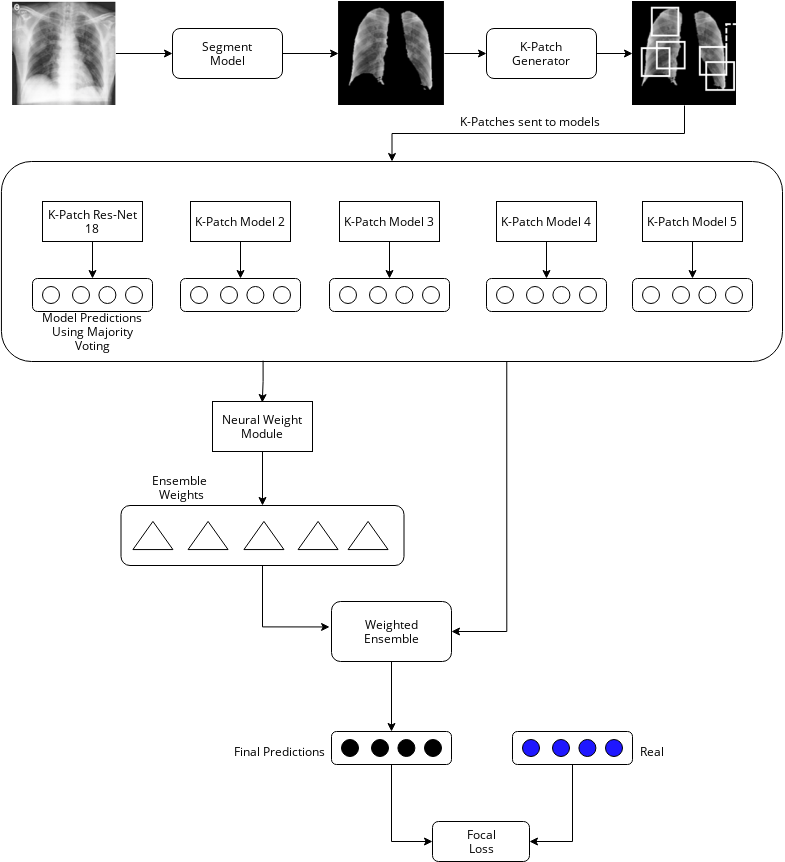
\includegraphics[width=8cm]{../doc/images/FLANNEL-IMPROVED.png}
\end{figure}


\section{Experimental Setup}
TODO
We are planning to use AWS for the training and evaluation.

\section{Timeline}


\begin{table}[H]
    \centering
    \caption{Project Timeline}
    \begin{tabular}{|c|c|} \hline
        Task&Planned Due Date\\ \hline
        Research, Planning and proposal &03/28/2021\\ \hline
        Data Cleaning and Preprocessing & 04/02/2021\\ \hline
        Extract the lung contours & 04/09/2021\\ \hline
        Apply classifier on each patch & 04/09/2021\\ \hline
        Ensemble the results from each classifier & 04/16/2021\\ \hline
        Calculate weights & 04/23/2021 \\ \hline
        Run the training data to get the prediction & 04/23/2021 \\ \hline
        Apply Focal Loss & 04/23/2021 \\ \hline
        Model Training & 04/23/2021 \\ \hline
        Performance Evaluation & 04/23/2021 \\ \hline
        Documentation and Video presentation & 05/07/2021 \\
        Code and Report Submission & 05/08/2021 \\
        \hline\end{tabular}
    \end{table}
    
    %
    % The following two commands are all you need in the
    % initial runs of your .tex file to
    % produce the bibliography for the citations in your paper.
    \bibliographystyle{abbrv}
    \bibliography{covid19}  % sigproc.bib is the name of the Bibliography in this case
    
    \end{document}
    